\documentclass[../../General.tex]{subfiles}
\begin{document}


\section{Módulo de sensores e instrumentación meteorológica}

\subsection{Selección del sensor de orientación absoluta primaria mediante unidad inercial integrada}

La alineación de la estación respecto a las directrices de la norma técnica internacional exige registrar la orientación espacial de la plataforma sobre el plano transversal con un margen de incertidumbre inferior a un grado. Para evitar el error producido por vibraciones mecánicas de rodadura, se demanda un sensor capaz de ejecutar internamente algoritmos de fusión y entregar cuaterniones o ángulos de Euler directamente por bus digital. En la Tabla \ref{tab:comp_imus} se confrontan tres módulos comerciales con nueve grados de libertad.

\begin{center}
    \renewcommand{\arraystretch}{1.5}
    \footnotesize
    \begin{xltabular}{\textwidth}{|p{3.5cm}|>{\centering\arraybackslash}X|>{\centering\arraybackslash}X|>{\centering\arraybackslash}X|}
        \caption{Tabla comparativa de unidades IMU de 9 ejes evaluadas\label{tab:comp_imus}} \\
        \hline
        \rowcolor[HTML]{D9E1F2} 
        \textbf{Parámetro Técnico} & \textbf{Opción A (Bosch BNO055)} & \textbf{Opción B (MPU-9250)} & \textbf{Opción C (ICM-20948)} \\ \hline
        \endfirsthead
        
        \multicolumn{4}{c}%
        {{\bfseries \tablename\ \thetable{} -- Continuación de la página anterior}} \\
        \hline
        \rowcolor[HTML]{D9E1F2} 
        \textbf{Parámetro Técnico} & \textbf{Opción A (Bosch BNO055)} & \textbf{Opción B (MPU-9250)} & \textbf{Opción C (ICM-20948)} \\ \hline
        \endhead
        
        \hline
        \endfoot
        
        \hline
        \endlastfoot
        
        Procesamiento de Fusión & Fusión por hardware en chip & Requiere librería externa & Procesador de movimiento parcial \\ \hline
        Precisión Angular Absoluta & Margen de medio grado & Margen de uno coma cinco grados & Margen de un grado \\ \hline
        Interfaz de Datos & Bus de dos hilos o serial & Bus de dos hilos o cuatro hilos & Bus de dos hilos o cuatro hilos \\ \hline
        Calibración de Sensores & Matriz dinámica en chip & Calibración manual en software & Calibración manual en software \\ \hline
        Tensión de Operación & Regulador integrado a 5.0 V & Tensión entre 2.4 V y 3.6 V & Tensión entre 1.71 V y 3.6 V \\ \hline
        Consumo de Corriente & 12.3 miliamperios & 3.5 miliamperios & 3.0 miliamperios \\ \hline
        Disponibilidad de Fabricación & Componente activo en catálogo & Obsoleto y discontinuado & Componente activo \\ \hline
    \end{xltabular}
\end{center}

Se selecciona el módulo Bosch BNO055. Su ventaja determinante consiste en integrar un procesador ARM Cortex-M0 que ejecuta el software propietario de fusión sensorial, entregando ángulos de inclinación, balanceo y guiñada en tiempo real con una precisión de $0.5^\circ$, reduciendo la carga computacional en los controladores del robot. El dispositivo se conecta a la línea de $5.0\text{ V}$ del bus I$^2$C en la dirección hexadecimal \texttt{0x28}.

\subsection{Arreglo de IMUs y traslación de niveles de voltaje}

Con el objeto de obtener retroalimentación de la posición de los sistemas de elevación y orientación, y brindar una referencia cinemática adicional para el movimiento del robots, se incorporan dos módulos basados en el transductor MPU-6050, integrando cada uno un acelerómetro y un giroscopio triaxiales de $16\text{ bits}$. 

A diferencia del sensor principal, los circuitos internos del transductor MPU-6050 operan estrictamente a $3.3\text{ V}$. Para comunicar ambos módulos con el bus de $5.0\text{ V}$ del microcontrolador sin degradar la pendiente de conmutación ni exponer los circuitos integrados a sobretensiones, se interpone un módulo traslador de nivel lógico bidireccional de 4 canales con transistores MOSFET. El lado de alta tensión del traslador se referencia a la barra de $5.0\text{ V}$ enlazándose a los terminales SDA y SCL del microcontrolador, mientras que el lado de baja tensión se referencia a la barra de $3.3\text{ V}$ comunicándose con las líneas de datos de los sensores.

Para permitir que ambos módulos coexistan en el mismo bus digital sin colisiones de arbitraje, la diferenciación de direcciones se implementa mediante cableado físico en la terminal de selección de dirección AD0. En el primer módulo, esta terminal se conecta a tierra GND para establecer la dirección hexadecimal \texttt{0x68}, mientras que en el segundo módulo se conecta a la barra de $3.3\text{ V}$ para fijar la dirección hexadecimal \texttt{0x69}. De esta manera, el sensor primario y los dos secundarios comparten el mismo bus a una velocidad de $400\text{ kHz}$.


%%%--------------------------------------------------------------------------------------------%%%
%%%--------------------------------------------------------------------------------------------%%%

\begin{figure}[H]
	% Fuerza la alineación izquierda y quita los ":" después del número
	\captionsetup{justification=raggedright, singlelinecheck=false, labelsep=none}
	
	\caption[.]{}
	
	\textit{.}\par\medskip
	
	\centering
	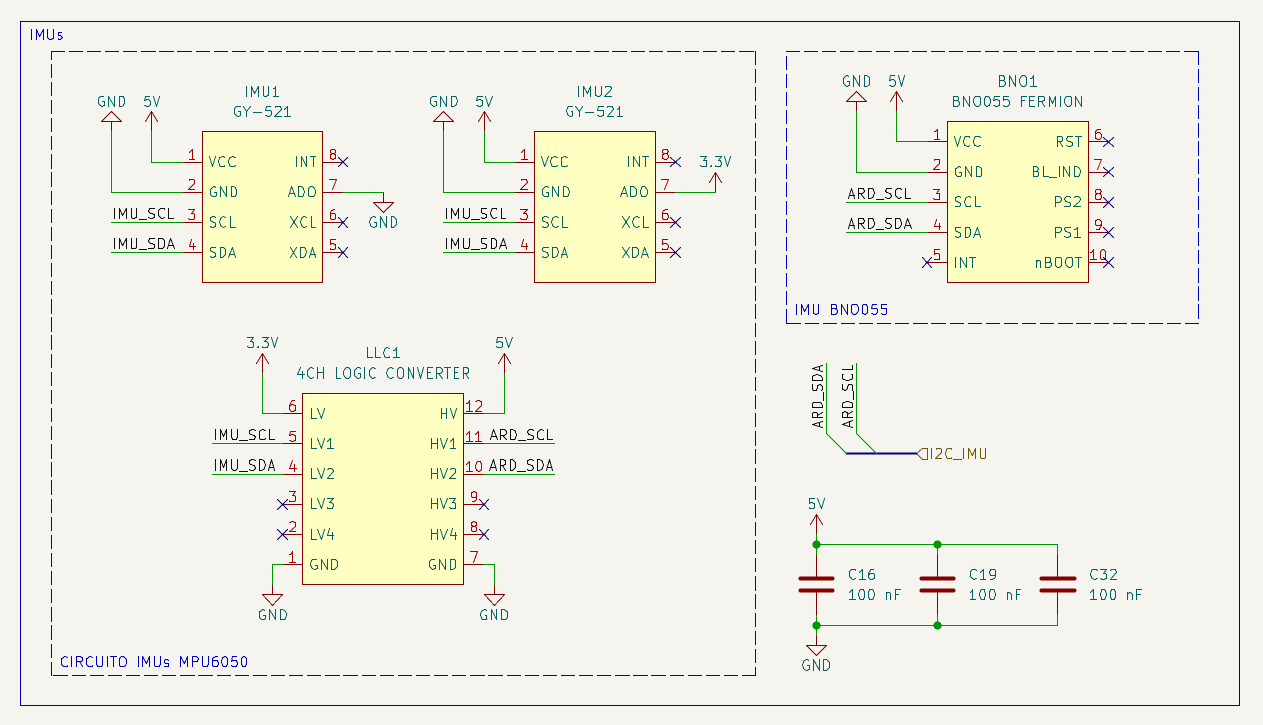
\includegraphics[width=0.75\textwidth]{Recursos/Imagenes/ImagenesDisenoElectronico/IMUArreglo.png} \par\medskip
	
	\raggedright
	\footnotesize \textit{Nota.} Elaboración propia.
	\label{fig:IMUArreglo}
\end{figure}

%%%
%%%--------------------------------------------------------------------------------------------%%%
%%%--------------------------------------------------------------------------------------------%%%

\subsection{Adquisición odométrica mediante encoder rotativo incremental}

La retroalimentación de la velocidad lineal y la posición del tren rodante se obtiene mediante un encoder óptico incremental de eje rotativo, modelo OMRON E6B2-CWZ6C. Este transductor incorpora emisores infrarrojos y un disco ranurado de alta precisión que entrega señales en cuadratura a través de sus canales A y B, acompañadas de un pulso de índice de referencia Z por cada vuelta mecánica completa.

La etapa de salida del encoder está configurada con transistores bipolares NPN a colector abierto que operan exclusivamente conmutando al potencial de masa, lo que permite independizar el potencial lógico de salida respecto a la alimentación de $24\text{ V}$ que recibe el dispositivo desde la barra filtrada. Las salidas se polarizan mediante resistencias pull-up de $1\text{ k}\Omega$ conectadas a la línea limpia de $5.0\text{ V}$, fijando los niveles en $0\text{ V}$ para el estado bajo y $5.0\text{ V}$ para el estado alto. La corriente de saturación resultante por canal es de $4.60\text{ mA}$, situándose muy por debajo del límite de $35\text{ mA}$ admitido por el componente. Considerando la capacitancia parásita de los conductores apantallados, el tiempo de subida de la señal se calcula en $0.264\mu\text{s}$, ocupando apenas el $5\%$ del semiciclo a la frecuencia máxima de $100\text{ kHz}$ y asegurando flancos nítidos sin transiciones espurias.

Con el fin de absorber la corriente transitoria de arranque de $9.0\text{ A}$ durante $0.3\text{ ms}$ especificada por el fabricante para el encendido del encoder, se dispone en los terminales de alimentación un filtro local formado por un condensador electrolítico de $47\text{ }\mu\text{F}$ en paralelo con un condensador cerámico de $100\text{ nF}$. Para decodificar la cuadratura en modo $4\times$ sin riesgo de pérdidas de pulsos por latencia de software, los canales A, B y Z se cablean directamente a las líneas de interrupción externa por hardware del microcontrolador en las terminales digitales 2, 3 y 8.

%%%--------------------------------------------------------------------------------------------%%%
%%%--------------------------------------------------------------------------------------------%%%

\begin{figure}[H]
	% Fuerza la alineación izquierda y quita los ":" después del número
	\captionsetup{justification=raggedright, singlelinecheck=false, labelsep=none}
	
	\caption[.]{}
	
	\textit{.}\par\medskip
	
	\centering
	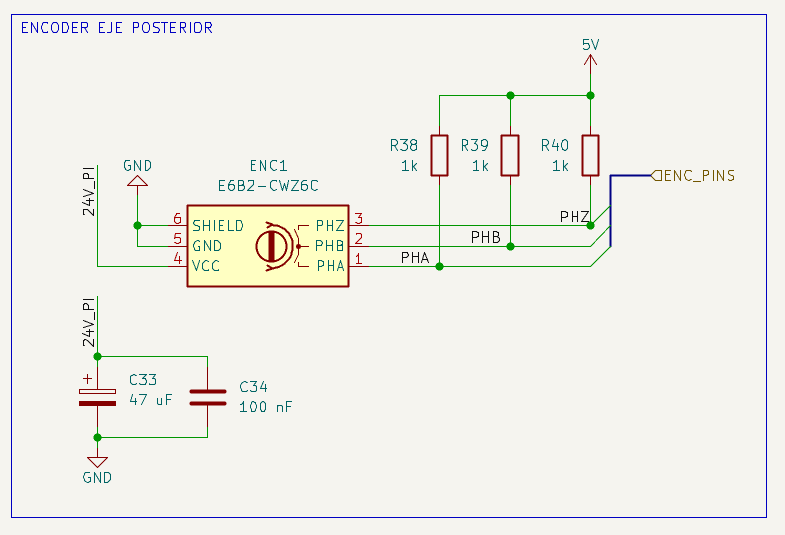
\includegraphics[width=0.75\textwidth]{Recursos/Imagenes/ImagenesDisenoElectronico/EncoderCircuit.png} \par\medskip
	
	\raggedright
	\footnotesize \textit{Nota.} Elaboración propia.
	\label{fig:EncoderCircuit}
\end{figure}

%%%
%%%--------------------------------------------------------------------------------------------%%%
%%%--------------------------------------------------------------------------------------------%%%

\subsection{Monitoreo de temperatura de la batería con termistor NTC}

El monitoreo térmico del gabinete electrónico y del chasis metálico se efectúa mediante un termistor NTC de contacto con terminal de arandela roscada (modelo NTCALUG02A), el cual presenta una resistencia nominal de $10\text{ k}\Omega$ a $25^\circ\text{C}$ y un coeficiente paramétrico ($\beta$) de $3984\text{ K}$.

El sensor conforma un divisor de voltaje alimentado desde la barra de $5.0\text{ V}$ junto a una resistencia de precisión de $10\text{ k}\Omega$ con tolerancia del $1\%$. En el nodo central del divisor se conecta un condensador cerámico de $100\text{ nF}$ a masa, integrando un filtro pasa bajas pasivo con una impedancia equivalente de $5\text{ k}\Omega$ y una frecuencia de corte calculada en $318.3\text{ Hz}$. Este filtro atenúa de forma eficaz el acoplamiento electromagnético procedente de los controladores de los motores antes de que la señal ingrese al ADC de $10\text{ bits}$ del microcontrolador en el canal analógico A0. En el software embebido, el valor digitalizado se procesa despejando la resistencia instantánea para calcular la temperatura mediante la ecuación del modelo Beta.


\subsection{Detección de límites mecánicos mediante sensores de fin de carrera}

La prevención de daños estructurales en los extremos de recorrido de los mecanismos de elevación y orientación se garantiza mediante interruptores mecánicos de fin de carrera con contactos normalmente abiertos acoplados a terminales de entrada digital del microcontrolador.

El circuito de acondicionamiento de cada interruptor se diseña con una resistencia de pull-down de $10\text{ k}\Omega$ conectada al nodo de señal, garantizando un potencial de $0\text{ V}$ cuando el interruptor permanece en reposo. Al conmutar el contacto hacia la barra de $5.0\text{ V}$ por presión mecánica del mecanismo, la línea se eleva a nivel alto provocando la lectura inmediata del estado. En paralelo con la resistencia de puesta a tierra se conecta una rama constituida por una resistencia limitadora de $330\Omega$ y un LED indicador, el cual se enciende con una corriente de $9\text{ mA}$ para brindar confirmación visual instantánea en la placa durante labores de calibración y mantenimiento sin afectar el umbral lógico digital. Las señales se asignan a las terminales digitales 31 y 32 del microcontrolador.

\begin{figure}[H]

	\captionsetup{justification=raggedright, singlelinecheck=false, labelsep=none}
	
	\caption[.]{} 
	
	\textit{.} \par\medskip
	
	\begin{minipage}{0.5\textwidth}
		\centering
		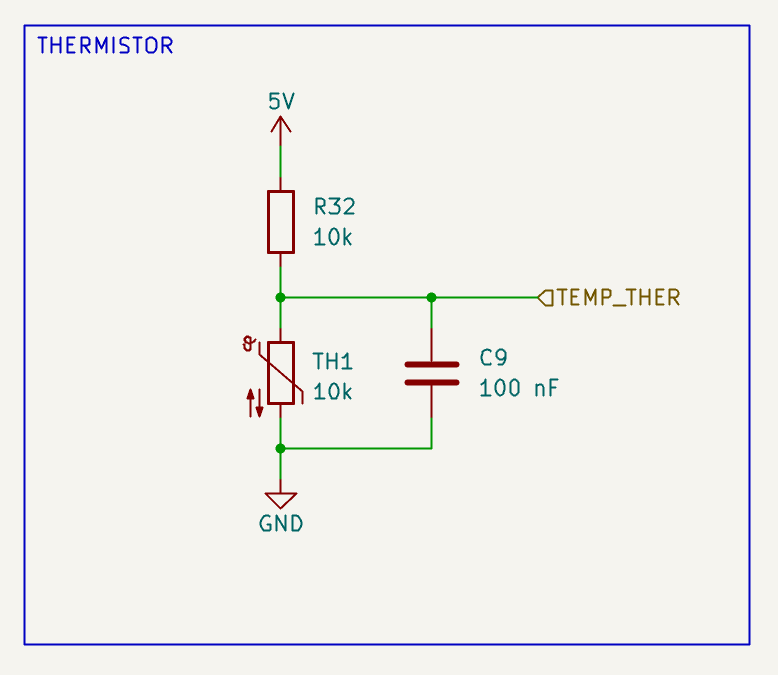
\includegraphics[width=\linewidth]{Recursos/Imagenes/ImagenesDisenoElectronico/ThermistorCircuit.png}
	\end{minipage}\hfill
	\begin{minipage}{0.5\textwidth}
		\centering
		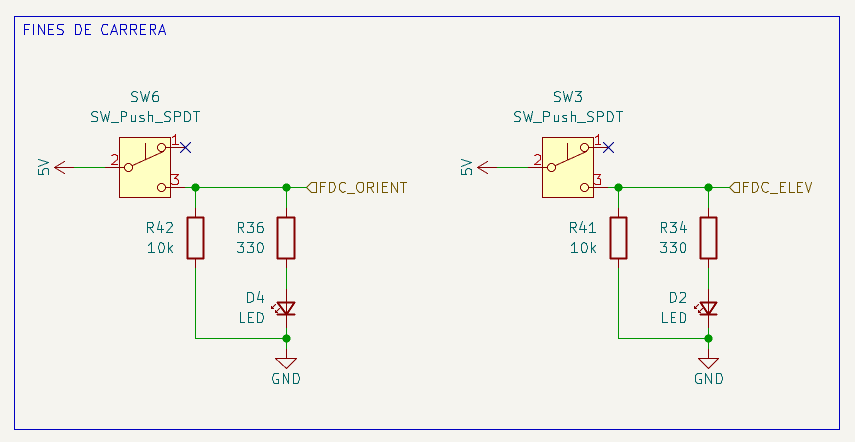
\includegraphics[width=\linewidth]{Recursos/Imagenes/ImagenesDisenoElectronico/FDCCircuit.png}
	\end{minipage}
	\par\medskip
	
	\raggedright
	\footnotesize \textit{Nota.} Elaboración propia.
	\label{fig:TermistorFDC}
\end{figure}

\end{document}